% !TEX encoding = UTF-8 Unicode

% This is a simple template for a LaTeX document using the "article" class.
% See "book", "report", "letter" for other types of document.

\documentclass[11pt]{article} % use larger type; default would be 10pt

\usepackage[utf8]{inputenc} % set input encoding (not needed with XeLaTeX)

%%% Examples of Article customizations

%%% PAGE DIMENSIONS
\usepackage{geometry} % to change the page dimensions
\geometry{a4paper} % or letterpaper (US) or a5paper or....
% \geometry{margin=2in} % for example, change the margins to 2 inches all round
% \geometry{landscape} % set up the page for landscape
%   read geometry.pdf for detailed page layout information

\usepackage{graphicx} % support the \includegraphics command and options

% \usepackage[parfill]{parskip} % Activate to begin paragraphs with an empty line rather than an indent

%%% PACKAGES
\usepackage{booktabs} % for much better looking tables
\usepackage{array} % for better arrays (eg matrices) in maths
\usepackage{paralist} % very flexible & customisable lists (eg. enumerate/itemize, etc.)
\usepackage{verbatim} % adds environment for commenting out blocks of text & for better verbatim
\usepackage{multicol,caption}
\usepackage{wrapfig}
\usepackage{parskip}
\usepackage{arydshln}
\usepackage{amsfonts}
\usepackage{amsmath}
\usepackage{hyperref}
% These packages are all incorporated in the memoir class to one degree or another...

%%% HEADERS & FOOTERS
\usepackage{fancyhdr} % This should be set AFTER setting up the page geometry
\pagestyle{fancy} % options: empty , plain , fancy
\renewcommand{\headrulewidth}{0pt} % customise the layout...
\lhead{}\chead{}\rhead{}
\lfoot{}\cfoot{\thepage}\rfoot{}

%%% SECTION TITLE APPEARANCE
\usepackage{sectsty}
\allsectionsfont{\sffamily\mdseries\upshape} % (See the fntguide.pdf for font help)
% (This matches ConTeXt defaults)

%%% ToC (table of contents) APPEARANCE
\usepackage[nottoc,notlof,notlot]{tocbibind} % Put the bibliography in the ToC
\usepackage[titles,subfigure]{tocloft} % Alter the style of the Table of Contents

\renewcommand{\cftsecfont}{\rmfamily\mdseries\upshape}
\renewcommand{\cftsecpagefont}{\rmfamily\mdseries\upshape} % No bold!
\newcommand{\squeezeup}{\vspace{-25pt}}

%%% Object appearance
\usepackage{float, makecell}
\usepackage{subcaption}
\newenvironment{Figure}{\par\medskip\noindent\minipage{\linewidth}}{\endminipage\par\medskip}
\newenvironment{Table}{\par\smallskip\noindent\minipage{\linewidth}}{\endminipage\par\smallskip}
\usepackage[linewidth=0.01pt,linecolor=black]{mdframed}
\captionsetup{justification=raggedright,singlelinecheck=false}


\hyphenation{ex-pe-ri-ences hy-per-pa-ra-me-ter com-pu-ta-tion-al-ly dis-cri-mi-na-tor}
%%% END Article customizations

%%% Document content

\title{Homework 1 : Unsupervised Deep Learning}
\author{João Ramos da Silva Tabuaço Freitas \\ Università Degli Studi di Padova \\ Student ID: 2009440}
\date{18 July 2022} %Display a given date

\begin{document}
\maketitle

\section*{Introduction}
Unsupervised learning takes an agnostic approach in learning features in data. This distinguishes it from supervised learning, where models attempt to form a connection between an input and a ground-truth target. The performance of unsupervised learning models is normally assessed by how faithfully data can be reproduced from the features learned.

\textbf{Autoencoders} and \textbf{generative-adversarial networks} (GANs) are two models used in unsupervised learning. In both cases, these models are composed by a perception module along with a reproduction module. These two work in tandem to achieve faithful reproduction of data with large number of features.

\noindent The goal of the autoencoder $A$ is to learn to embed input data $\mathbf{x}$ in a latent space $\mathbb{R}^{n}$ of reduced dimensionality, and subsequently reproduce it. To achieve this, an encoder $E$ transforms an input $\mathbf{x}$ into a vector $z = E(\mathbf{x}), z \in \mathbb{R}^{n}$. A decoder $D$ then attempts to reproduce the original input $\mathbf{x}' = D(z)$ as faithfully as possible. This motivates the use of mean-squared error (MSE) to quantify the reconstruction error.

\begin{equation}
    \{\hat{w}\}= \arg\min_{w} \frac{1}{n}\sum_{i = 1}^{n}\left(\hat{\mathbf{x}}_i - \mathbf{x}_i\right)^{2}
\end{equation}

\noindent Of course, the autoencoder $A := D \circ E$.

\noindent Autoencoders with a latent space of lower dimension than the input space are said to be undercomplete, while those with a larger latent space are overcomplete. The former performs dimensionality reduction, by learning only data's most prominent features. This proves useful in denoising input, for example. While the latter could have the capability of capturing larger detail from the inputs, its learning converges to the identity. While this achieves the lowest reconstruction error, it has little practical value.

\noindent The performance of an undercomplete autoencoder can be assessed qualitatively by how well it manages to separate the different categories of the data in the latent space. To visualize this, principal component analysis (PCA) and t-distributed stochastic neighbor embedding (t-SNE) are used to further reduce the dimensionality of the latent vectors.

\noindent The structure of a GAN starts with a generator which produces samples $\mathbf{x} = g(\mathbf{z},w_{g})$ from a randomly generated latent vector $\mathbf{z}$, where $w_{g}$ are the generator parameters. These samples are then fed into the discriminator, whose goal is to observe an input, and reach a conclusion $y = d(\mathbf{x}, w_{d}) = d(g(\mathbf{z},w_{g}), w_{d})$ about said input (with $w_{d}$ being the discriminator parameters). The learning task can be formulated as a zero-sum game solved by a minimax decision.\footnote{Goodfellow, I. J., Pouget-Abadie, J., Mirza, M., Xu, B., Warde-Farley, D., Ozair, S.,
Courville, A., and Bengio, Y. (2014c). Generative adversarial networks. In NIPS’2014.} The discriminator observes a payoff $v(g, d)$, while the generator receives $-v(g,d)$. Thus, the goal is to find $g^*$ such that:

\begin{equation}
    g^* = \arg\min_{g}\max_{d} v(g,d)
\end{equation}

Normally, the choice of $v(g, d)$ is:
\begin{equation}
    v_{\text{mm}}(g,d) = - \mathbb{E}_{\mathbf{x}\sim p_{\text{data}}}[\log(d(\mathbf{x}))] - \mathbb{E}_{\mathbf{x}\sim p_{g}}[\log(1 - d(\mathbf{x}))]
\end{equation}

In other words, the aim of the minimax game is for the discriminator to maximize its payoff by classifying fake/real inputs correctly, while the generator attempts to minimize the discriminator's payoff by tricking it into believing that the inputs are real.

\noindent One issue with the minimax game formulation is that the gradient quickly diverges away from $d(\mathbf{x}) = 1/2$. This can be addressed by modifying the generator loss, as is done in non-saturating GAN (NSGAN) formulation.\footnote{Lucic, M., Kurach, K., Michalski, M., Bousquet, O., Gelly, S.,  (2018). Are GANs Created Equal? A Large-Scale Study. In NIPS'2018.} In this scenario, the discriminator loss is the same as $v_{\text{mm}}$, while the generator loss is:
\begin{equation}
    v_{\text{NS}}(g,d) = - \mathbb{E}_{\mathbf{x}\sim p_{g}}[\log(d(\mathbf{x}))]
\end{equation}

Both the minimax and the non-saturating formulations will be explored.

%%%%%%%%%%%%%%  Methods section %%%%%%%%%%%%%%
\section*{Methods}

The FashionMNIST dataset is used to explore both the autoencoder and the GAN, with each image having shape $\left(1, 28, 28\right)$. The set used for training consisted of $60000$ equally distributed samples, which was sectioned to serve the purpose of validation as well. The test set consists of $10000$ samples with the same properties. 
 
The autoencoder architecture consists of three convolutional layers, followed by two fully connected layers. Regularization is implemented through batch normalization on the convolutional layers, and L2 penalty on the loss. The number of convolutional filters, number of fully-connected neurons, optimizer algorithm, and learning rate are tuned using Optuna, which attempted $20$ sets of parameters, training each model over five epochs. The latent space dimension is also tuned, but kept below $15$ to curb overfitting. The convolutional kernel sizes, strides and padding are kept constant to preserve the same output shapes in all trials.

\noindent Upon tuning the model architecture, the model was validated using a K-Fold cross-validation strategy, splitting the dataset in six sequential folds and performing training over $20$ epochs. The performance was assessed based on the reconstruction error on the test set.

\noindent To test the expressive power of the model, a convolutional neural network was trained to classify the set of latent vectors corresponding to the input data. The network's learning curve was compared to a similar network trained on the unaltered dataset, over $50$ epochs.

\noindent The latent space was reduced to three dimensions using PCA and also t-SNE. A well-performing encoder should be able to keep the different classes spatially separated. Of course, some confusion is expected between classes of similar-looking items, regardless of the method used for reducing dimensionality. 

\noindent The creation and training of the GAN posed several challenges. The level of complexity of the model discouraged hyperparameter tuning. This was because the Optuna framework would have to explore the hyperparameter space based on two different metrics (generator and discriminator loss). The set of parameters which would improve the generator performance could hinder the discriminator's, and vice-versa. Because of this, automated tuning was not performed. Furthermore, the training process revealed itself demanding from a computational standpoint. As a result, only one model was trained without cross-validation. Given the well-known regularity of the FashionMNIST dataset, this is acceptable, as there are no large disparities in different sections of the dataset.

\noindent Both components of the GAN were endowed with four convolutional layers, and no fully-connected section. The number of filters, kernel sizes, strides, and padding were chosen in order to have the generator outputting an image with the same dimensions as the FashionMNIST inputs, and the discriminator outputting a single scalar value.

\section*{Results}



\noindent The best architecture found for the autoencoder is described in Table \ref{tab:AE_params}. The K-fold results (Figure \ref{fig:kfold}) show little variability in the learning curves, which is expected by the fairly regular nature and even distribution of class labels in the dataset. 

\begin{wraptable}{l}{9cm}
    %%% AE_params table
\resizebox{0.6\textwidth}{!}{%
    \begin{tabular}{ccccccc}
        Layer & \thead{No. channels \\ Neurons} & \thead{(Kernel,\\ Strides,\\ Padding)} & Activation & \thead{Batch \\ Normalization}\\
        \hline
        \textsc{conv1} & 7 & (3, 2, 1) & ReLU & Yes\\
        \textsc{conv2} & 32 & (3, 2, 1) & ReLU & Yes\\
        \textsc{conv3} & 43 & (3, 2, 0) & ReLU & Yes\\
        \textsc{Lin1} & 87 & N/A & ReLU & N/A \\
        \hdashline
        \textsc{Latent} & 15 & N/A & N/A & N/A \\
        \hdashline
        \textsc{Lin1} & 87 & N/A & ReLU & N/A \\
        \textsc{deconv1} & 43 & (3, 2, 0) & ReLU & Yes\\
        \textsc{deconv2} & 32 & (3, 2, 1) & ReLU & Yes\\
        \textsc{deconv3} & 7 & (3, 2, 1) & ReLU & Yes\\
    \end{tabular}}
    \caption{Autoencoder architecture. The number of channels in \textsc{conv[i]} corresponds to output channels, while it corresponds to input channels in \textsc{Deconv[i]}.}
    \label{tab:AE_params}
\end{wraptable}

While the training loss experiences larger variance, the trend is similar for training and validation across all folds. The convergence of training and validation loss close to 20 training epochs indicates the model is well-regularized and not overfitting.

\begin{wrapfigure}{r}{7cm}
    \centering
    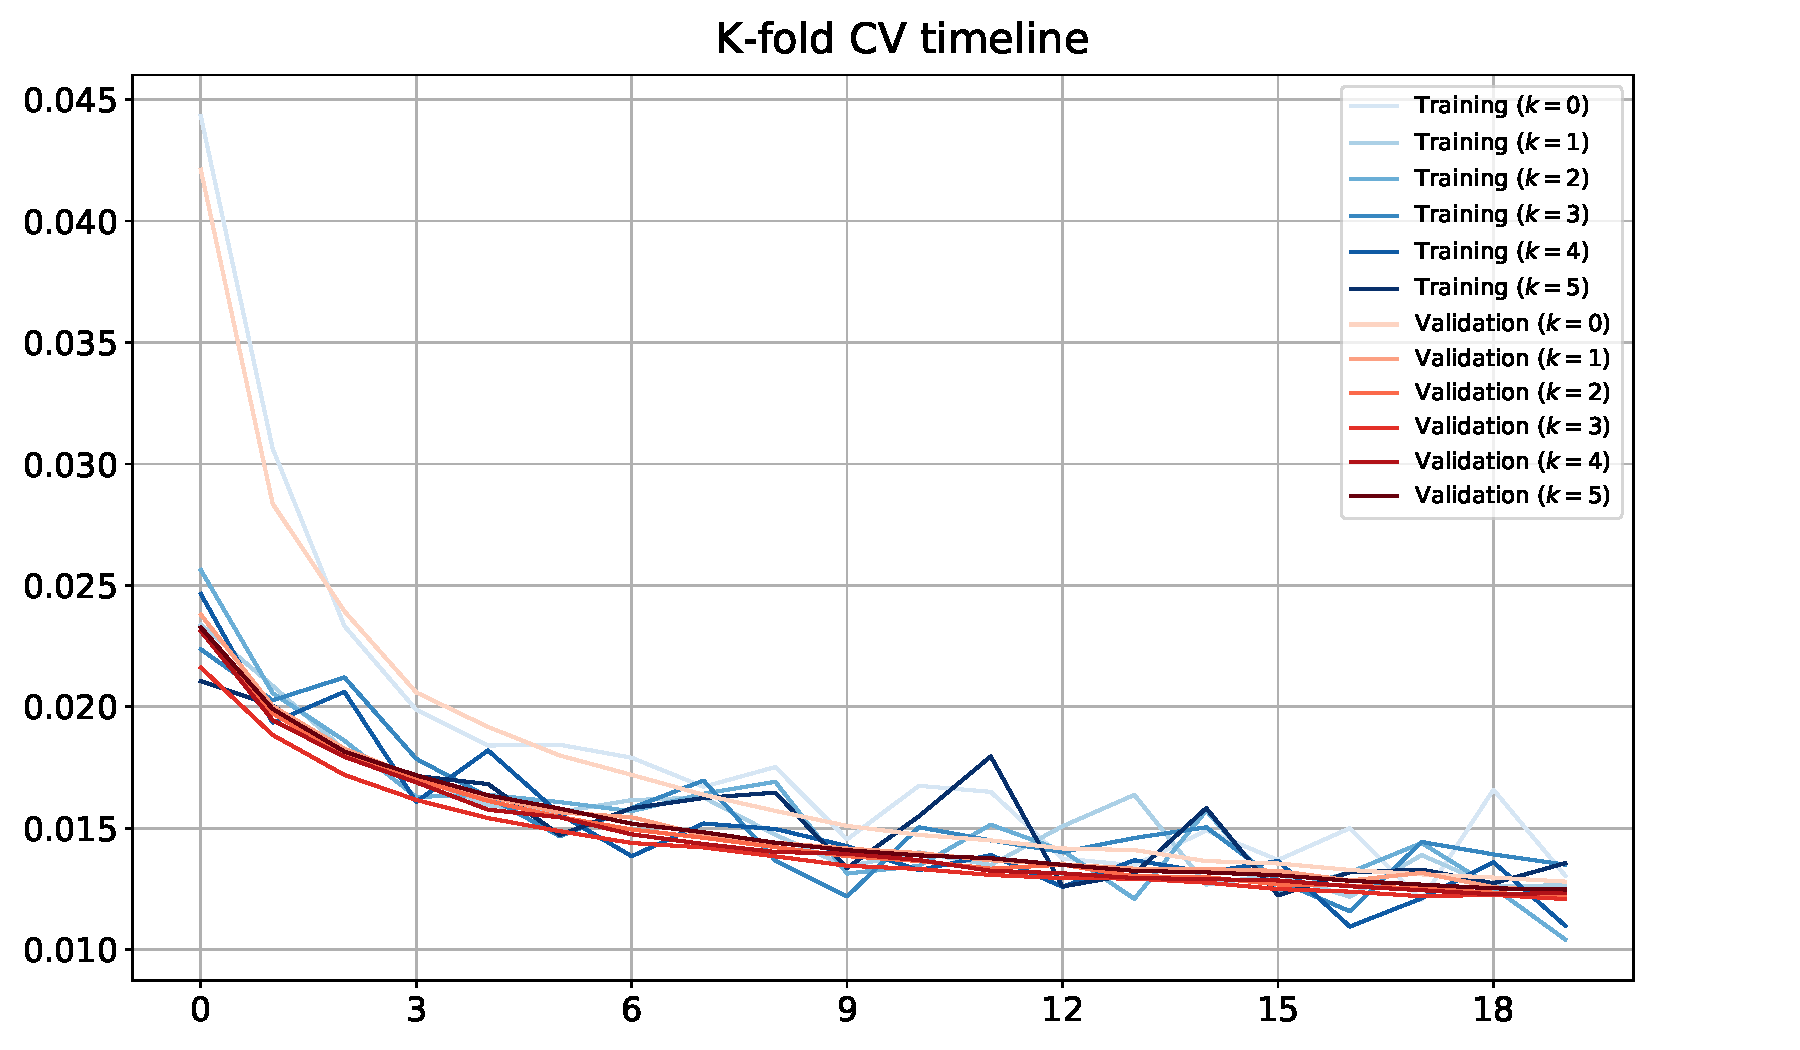
\includegraphics[width=0.52\textwidth]{res/learning_curve_KFCV.pdf}
    \caption{K-fold learning curves.}
    \label{fig:kfold}
\end{wrapfigure}

\noindent The denoising capabilities of the autoencoder were tested by inputting an image with different levels of noise. One sample image is reconstructed (Figure \ref{fig:recon}), and the loss was shown to improve in all extents of noise tested. However, this is not always the case, and generally depends on the sample used. Samples with a larger number of blackened pixels on their own are less likely to see an improvement. This is because the choice of blackened pixels is uniformly random, so the noisy sample might have stayed very similar to the original. The model struggled more to reconstruct samples when Gaussian noise was added. This could be attributed to the lack of noisy samples in the training process, and was left out of the analysis.

\noindent Two classifier models were separately trained on the original dataset and on the corresponding latent space version produced by the autoencoder. The learning curves were compared (Figure \ref{fig:classifier}). The difference in the loss seems consistent throughout the training process. Still, both sets of data lead to a stable learning curve which converges in similar time. Of course, the classifiers used were fully connected networks, which underperform when compared with convolutional networks for image classification. However, the training with the encoded data is visibly faster, with the classification on the encoded set having taken $369$ seconds, and the classification on the original set taking $725$ seconds. Thus, with limited computational resources, the latent space representation achieved by the autoencoder can speed up the training process of a classifier.

\begin{figure}[t]
    \centering
    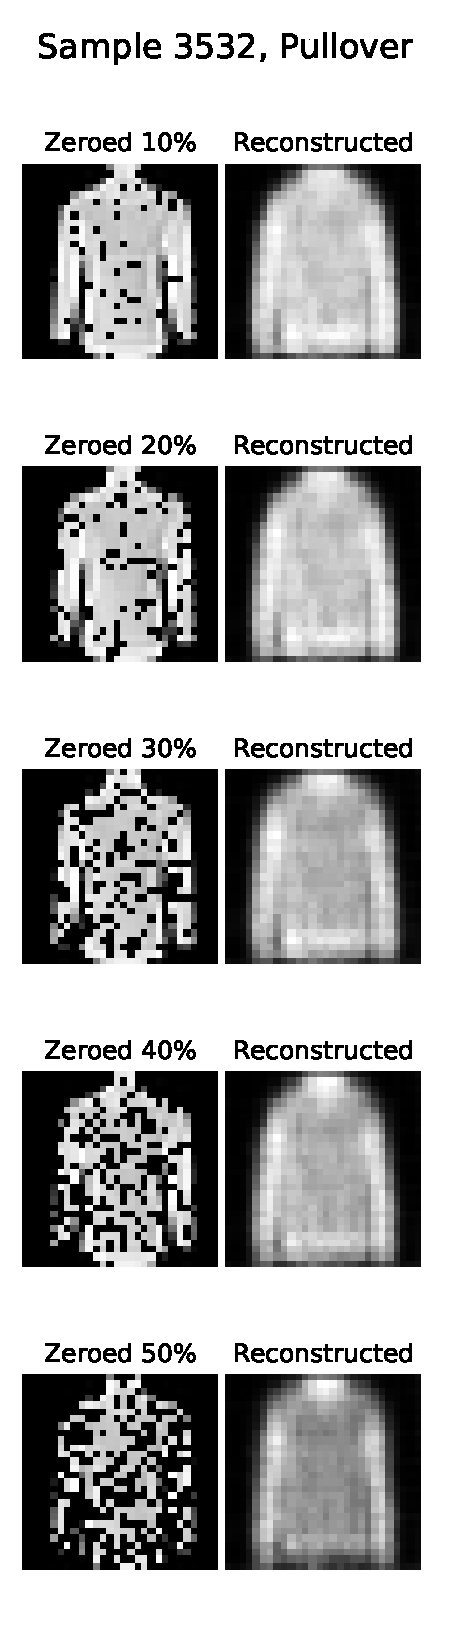
\includegraphics[width=\textwidth]{res/Reconstruction.pdf}
    \caption{Sample reconstruction.}
    \label{fig:recon}
\end{figure}

\begin{figure}[t]
    \centering
    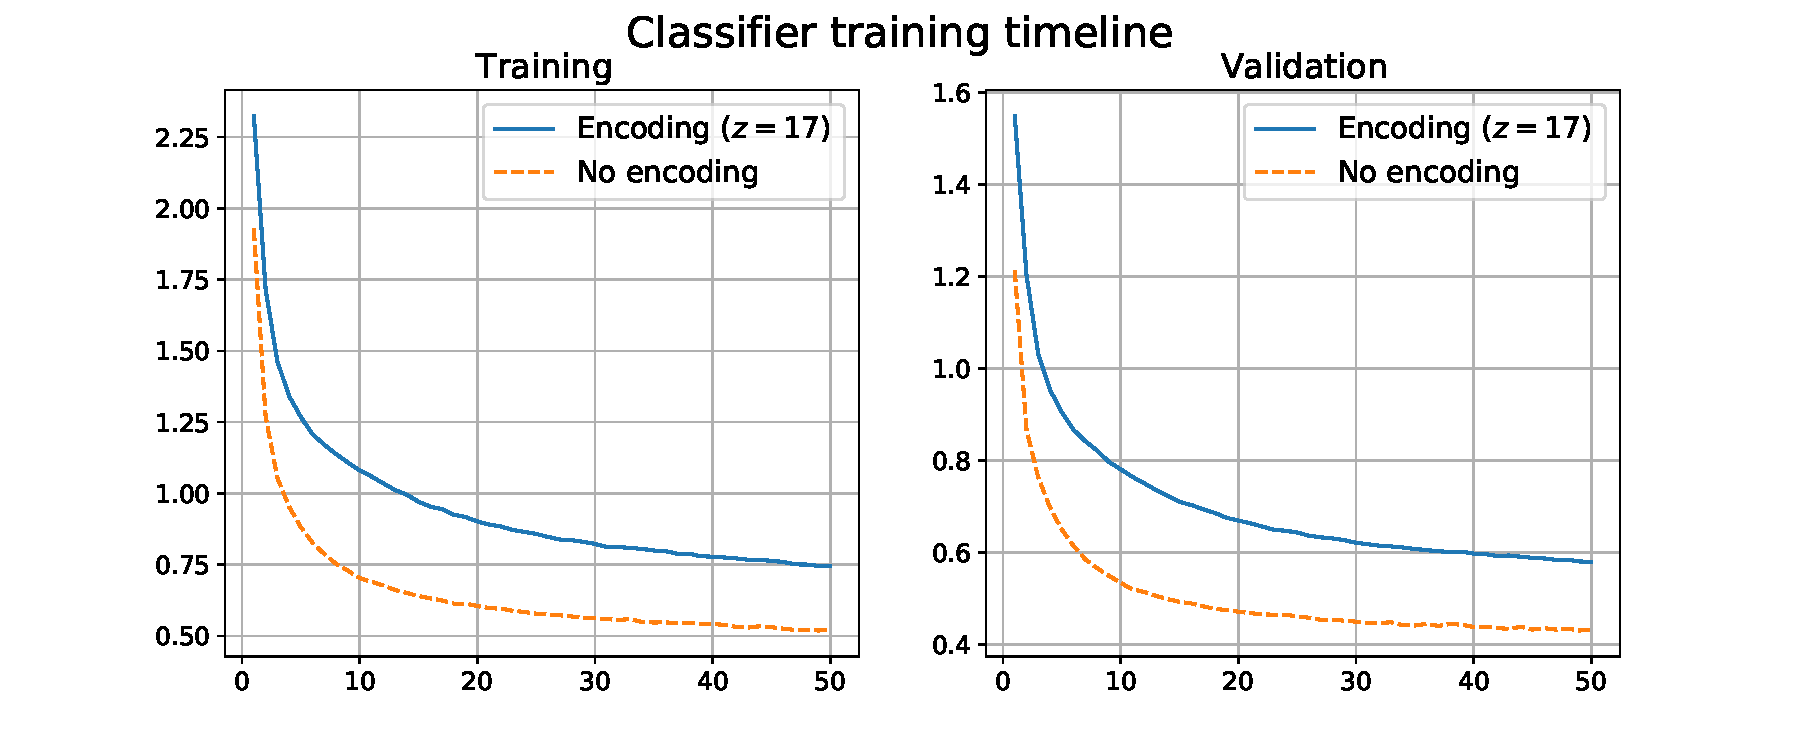
\includegraphics[width=\textwidth]{res/classifier_lcurve.pdf}
    \caption{Classifier learning curves.}
    \label{fig:classifier}
\end{figure}

Interactive plots for \href{run:res/pca_plot.html}{PCA} and \href{run:res/tsne_plot.html}{t-SNE}\footnote{Clicking on "PCA" or "t-SNE" will open the respective plot.} have been generated using plotly. They show an acceptable clustering. While both algorithms managed to cluster the latent vectors with low variance, t-SNE outperformed PCA in separating classes with distinct features (e.g. hand bags or trousers). Furthermore, the FashionMNIST dataset contains several upper body clothing items, which share similar visual features among themselves. These are generally the data with higher associated classification loss. Both methods also struggle to keep these classes separated.

\pagebreak

The formulation of the GAN as a minimax game complicates the hyperparameter search, because the optimization must take place in two opposite directions simultaneously. This requires a larger search space, which proved to be too computationally demanding. Furthermore, most attempts lead to an overtrained discriminator that hinders the learning in the generator. Because of this, hyperparameter optimization was not carried out for this model. The two models were trained over 30 epochs each, with identical architectures, learning rates and optimizers.

\begin{wraptable}{r}{7.4cm}
    \begin{tabular}{c|cc}
        Sample type & Minimax & Non-saturating\\
        \hline
        Real set & 0.7422 & 0.6943\\
        Fake set & 2.0723 & 1.5302\\
        
    \end{tabular}
    \caption{Discriminator test results (30 epochs).}
    \label{tab:GAN_results30}
\end{wraptable}

GANs were trained using both a minimax and a non-saturating criteria. The performance of the generator can only really be benchmarked by the discriminator's ability to distinguish between real and fake samples.  The test results are reported in Table \ref{tab:GAN_results30}. The discriminator trained with the non-saturating variation performs slightly better than the minimax variant. The performance of the generator can be further explored visually. Using a latent vector of random noise, the two models can be compared by the realness of the generated images. Based on the lack of detail observed in the non-saturating case, we can see that the lower performance of the minimax discriminator is likely a consequence of a more well-trained generator. The output of the non-saturating generator is not as clear as with the minimax case.

\begin{wraptable}{r}{7.4cm}
    \begin{tabular}{c|cc}
        Sample type & Minimax & Non-saturating\\
        \hline
        Real set & 0.5029 & 0.5677\\
        Fake set & 1.4158 & 1.3403\\
        
    \end{tabular}
    \caption{Discriminator test results (80 epochs).}
    \label{tab:GAN_results80}
\end{wraptable}

In order to further explore the performance of the non-saturating GAN, the models were re-trained over 80 epochs (Table \ref{tab:GAN_results80}). Naturally, both discriminators display an improved performance. The non-saturating discriminator shows a bias towards classifying fake samples, which is illustrated by a higher loss in the real samples, and a lower loss in the fake samples. The minimax discriminator shows a better capability in discerning real images, but performs slightly worse in discerning fakes. This might indicate a better trained generator. In either case, it is clear that convergence of the GAN model requires very long training times. While non-saturating frameworks might achieve better results earlier in the training process, performance seems to be similar in the long run.

\end{document}